\documentclass{article}
\usepackage[top=3cm, bottom=3cm, left = 2cm, right = 2cm]{geometry} 
\geometry{a4paper} 
\usepackage[T1]{polski}
\usepackage[utf8]{inputenc}
\usepackage{titling}
\usepackage{caption}
\usepackage{algorithm}
\usepackage{algpseudocode}
\usepackage[parfill]{parskip}
\usepackage{multirow}
\usepackage{graphicx}

\renewcommand\maketitlehooka{\null\mbox{}\vfill}
\renewcommand\maketitlehookd{\vfill\null}

\floatname{algorithm}{Algorytm}
\algrenewcommand\algorithmicrequire{\textbf{Input:}}
\algrenewcommand\algorithmicensure{\textbf{Output:}}

\title{Obliczenia Naukowe}
\author{Karol Janic}
\date{21 października 2023}

\begin{document}

\begin{titlingpage}
    \maketitle
\end{titlingpage}

\tableofcontents

\newpage

\section{Zadanie 1}
\subsection{Cel}
Celem zadania jest wyznaczenie liczb:
\begin{itemize}
    \item \texttt{macheps} - najmniejszej liczby, takiej że $fl(\texttt{1.0 + macheps}) > 1.0$ oraz $fl(\texttt{1.0 + macheps}) = 1.0 + \texttt{macheps}$
    \item \texttt{eta} - najmniejszej dodatniej liczby
    \item \texttt{max} - największej reprezentowalnej liczby
\end{itemize}
w arytmetykach 16-, 32- oraz 64-bitowej, porównanie ich wartości z wartościami zwracanymi przez wbudowane funkcje w języku \texttt{Julia} oraz wartościami zdefiniowanymi w języku \texttt{C}.
Dodatkowo należy ocenić związki \texttt{macheps} z precyzją arytmetyki, $MIN_{sub}$ z \texttt{eta}, $MIN_{nor}$ z wbudowaną funkcją języka \texttt{Julia} \texttt{floatmin} oraz $MAX$ \newline z \texttt{floatmax}. Określone są one przez wzory:

\subsection{Rozwiązanie}
Wymienione powyżej liczby obliczane są w sposób iteracyjny. Obliczenie wykonywane są w arytmetyce zmiennopozycyjnej:
\begin{itemize}
    \item \texttt{macheps} inicjalizowany jest wartością $1.0$ a następnie połowiony do momentu aż dodanie jego połowy do $1.0$ nie da w wyniku liczby większej niż $1.0$
    \item \texttt{eta} inicjalizowana jest wartością $1.0$ a następnie połowiona dopóki jego połowa jest większa od $0.0$
    \item \texttt{max} inicjalizowany jest wartością $1.0$ a następnie podwajany dopóki jego podwojona wartośc nie będzie nieskończonością. Następnie jest powiększany o coraz mniejsze liczby dopóki dodanie kolejnej liczby nie spowoduje osiągnięcia nieskończoności
\end{itemize}

\begin{algorithm}
    \caption{Wyznaczanie \texttt{macheps}}
    \begin{algorithmic}
    \State $macheps \gets 1.0$
    \While{$fl(1.0 + \frac{macheps}{2}) > 1.0 $}
        \State $macheps \gets \frac{macheps}{2}$
    \EndWhile
    \end{algorithmic}
\end{algorithm}

\begin{algorithm}
    \caption{Wyznaczanie \texttt{eta}}
    \begin{algorithmic}
        \State $eta \gets 1.0$
        \While{$fl(\frac{eta}{2}) > 0.0$}
            \State $eta \gets \frac{eta}{2}$
        \EndWhile
    \end{algorithmic}
\end{algorithm}

\begin{algorithm}
    \caption{Wyznaczanie \texttt{max}}
    \begin{algorithmic}
        \State $max \gets 1.0$
        \While{$fl(2 * max) \neq \infty$}
            \State $max \gets 2 * max$
        \EndWhile

        \State $gap \gets \frac{max}{2}$

        \While{$fl(max + gap) \neq \infty$ and $fl(gap) > 0.0$}
            \State $max \gets max + gap$
            \State $gap \gets \frac{gap}{2}$
        \EndWhile
    \end{algorithmic}
\end{algorithm}

\subsection{Wyniki i wnioski}
Wartości \texttt{macheps} wyznaczone przy użyciu opisanego wyżej algorytmu pokrywają się z wartościami otrzymanymi z wbudowanych funkcji języka \texttt{Julia} oraz są bliskie stałymi w języku \texttt{C} (za wyjątkiem 16-bitowej reprezentacji, której język \texttt{C} nie zapewnia).
\begin{table}[h!]
    \centering
    \begin{tabular}{ |c|c|c|c| } 
    \hline
    typ & wartość wyznaczona & wartość \texttt{eps} w \texttt{Julii} & wartość w \texttt{float.h} w \texttt{C} \\ 
    \hline
    \texttt{Float16} & 0.000977 & 0.000977 & niezdefiniowana \\ 
    \hline
    \texttt{Float32} & 1.1920929e-7 & 1.1920929e-7 & 1.192093e-7 \\ 
    \hline
    \texttt{Float32} & 2.220446049250313e-16 & 2.220446049250313e-16 & 2.220446e-16 \\ 
    \hline
    \end{tabular}
    \caption{Porównanie wartości \texttt{macheps}.}
\end{table}
\newline
Prezycję ayrtmetyki $\epsilon$ określa formuła: 
\begin{center}
    $\epsilon = \frac{1}{2} \beta^{t - 1}$,
\end{center}
gdzie $\beta$ jest bazą rozwinięcia, a $t$ liczbą cyft użytych do zapisu mantysy. Dla typów \texttt{Float16}, \texttt{Float32}, \texttt{Float64} $\beta = 2$ a $t$ przyjmuje kolejno wartości $10$, $23$, $52$. Łatwo można sprawdzić, że wartości \texttt{macheps} pokrywają się \newline z prezycją arytmetyki.
\newline
\begin{table}[h!]
    \centering
    \begin{tabular}{ |c|c|c| }
        \hline
        typ & \texttt{macheps} & $\epsilon$ \\
        \hline
        \texttt{Float16} & 0.000977 & 0.000977 \\
        \hline 
        \texttt{Float32} & 1.1920929e-7 & 1.1920929e-7 \\
        \hline
        \texttt{Float64} & 2.220446049250313e-16 & 2.220446049250313e-16 \\
        \hline
    \end{tabular}
    \caption{Porównanie wartości \texttt{macheps} z $\epsilon$.}
\end{table}
\newline
Wartości \texttt{eta} wyznaczone przy użyciu opisanego wyżej algorytmu pokrywają się z wartościami otrzymanymi \newline z wbudowanych funkcji języka \texttt{Julia}. Język \texttt{C} nie definiuje takiej stałej.
\begin{table}[h!]
    \centering
    \begin{tabular}{ |c|c|c| } 
    \hline
    typ & wartość wyznaczona & wartość \texttt{nextfloat(Typ(0.0))} w \texttt{Julii} \\ 
    \hline
    \texttt{Float16} & 6.0e-8 & 6.0e-8 \\ 
    \hline
    \texttt{Float32} & 1.0e-45 & 1.0e-45 \\ 
    \hline
    \texttt{Float64} & 5.0e-324 & 5.0e-324 \\ 
    \hline
    \end{tabular}
    \caption{Porównanie wartości \texttt{eta}.}
\end{table}
\newline
$MIN_{sub}$ jest najmiejszą dla arytmetyki nieznormalizowaną liczbą.  $MIN_{nor}$ jest najmniejszą dla arytmetyki znormalizowaną liczbą.

\begin{center}
    $MIN_{sub} = 2^{1-t} \cdot 2^{c_{min}}$

    $MIN_{nor} = 2^{c_{min}}$,
\end{center}
gdzie $c_{min}$ jest minimalną możliwą do zapisania cechą wyznaczaną ze wzoru:
\begin{center}
    $c_{min} = -2^{d - 1} + 2$,
\end{center}
gdzie $d$ jest liczbą bitów przeznaczonych na zapis cechy. Dla typów zmiennopozycyjnych \texttt{Float16}, \texttt{Float32}, \texttt{Float64} są to kolejno $5$, $8$, $11$.
\begin{table}[h!]
    \centering
    \begin{tabular}{ |c|c|c|c|c| }
    \hline 
    typ & \texttt{eta} & $MIN_{sub}$ & $MIN_{nor}$ & \texttt{floatmin(typ)} \\
    \hline
    \texttt{Float16} & 6.0e-8 & 6.0e-8 & 6.104e-5 & 6.104e-5 \\
    \hline
    \texttt{Float32} & 1.0e-45 & 1.0e-45 & 1.1754944e-38 & 1.1754944e-38 \\
    \hline
    \texttt{Float64} & 5.0e-324 & 5.0e-324 & 2.2250738585072014e-308 & 2.2250738585072014e-308 \\
    \hline
    \end{tabular}
    \caption{Porównanie wartości \texttt{eta}, $MIN_{sub}$, $MIN_{nor}$ oraz \texttt{floatmin}.}
\end{table}

\newpage 

Z powyższych obliczeń wynika, że wartość $MIN_{sub}$ jest równa \texttt{eta} a $MIN_{nor}$ \texttt{floatmin}. Można zauważyc, że wartości $MIN_{nor}$ są większe od wartości $MIN_{sub}$.

Wartości \texttt{max} wyznaczone przy użyciu opisanego wyżej algorytmu pokrywają się z wartościami otrzymanymi z wbudowanych funkcji języka \texttt{Julia} oraz są bliskie stałymi w języku \texttt{C} (za wyjątkiem 16-bitowej reprezentacji, której język \texttt{C} nie zapewnia).

\begin{table}[h!]
    \centering
    \begin{tabular}{ |c|c|c|c| } 
    \hline
    typ & wartość wyznaczona & Wartość \texttt{floatmax(typ)} w \texttt{Julii} & wartość w \texttt{float.h} w \texttt{C} \\ 
    \hline
    \texttt{Float16} & 6.55e4 & 6.55e4 & niezdefiniowana \\ 
    \hline
    \texttt{Float32} & 3.4028235e38 & 3.4028235e38 & 3.402823e38 \\ 
    \hline
    \texttt{Float64} & 1.7976931348623157e308 & 1.7976931348623157e308 & 1.797693e308 \\ 
    \hline
    \end{tabular}
    \caption{Porównanie wartości \texttt{max}.}
\end{table}

\section{Zadanie 2}
\subsection{Cel}
Celem zadania jest sprawdzenie poprawności wzoru Kahana na wartość epsilona maszynowego. Przedstawił on następujący wzór:
\begin{center}
    $\epsilon_{Kahan} = 3 \cdot (\frac{4}{3} - 1) - 1$
\end{center}

\subsection{Rozwiązanie}
Zaimplementowano funkcję wzracającą wartość epsilona przedstawioną przez Kahana. Dla różnych typów danych wygenerowano ją oraz porównano z wartościami \texttt{macheps}. 

\subsection{Wyniki i wnioski}
Z przeprowadzonych obliczeń wynika, że wartości obliczone na podstawie wzoru Kahana różnią się wyłącznie znakiem od wartości \texttt{macheps}.

\begin{table}[h!]
    \centering
    \begin{tabular}{ |c|c|c| }
    \hline
    typ & \texttt{macheps} & $\epsilon_{Kahan}$ \\
    \hline
    \texttt{Float16} & 0.000977 & -0.000977 \\
    \hline
    \texttt{Float32} & 1.1920929e-7 & 1.1920929e-7 \\
    \hline
    \texttt{Float64} & 2.220446049250313e-16 & -2.220446049250313e-16 \\
    \hline
    \end{tabular}
    \caption{Porównanie wartości \texttt{macheps} z wartościami obliczonymi ze wzoru Kahana.}
\end{table}
\section{Zadanie 3}
\subsection{Cel}
Celem zadania jest sprawdzenie, czy liczby w arytmetyce zmiennopozycyjnej \texttt{Float64} są równomiernie rozłożone w przedziale $[1, 2]$ z krokiem $\delta = 2^{-52}$ oraz w przedziałach $[\frac{1}{2}, 1]$ i $[2, 4]$.
\subsection{Rozwiązanie}
W celu odpowiedzi na powyższe pytanie w podanych przedziałach generowano kolejne liczby w arytmetyce \texttt{Float64} na dwa różne sposoby oraz porównano je. Jednym z nich jest dodawanie $\delta$ zaś drugim zwiekszanie liczby reprezentującej mantysę o jeden.

\subsection{Wyniki i wnioski}
W wyniku działania programu dla przedziału $[1, 2]$ nie wykryto rozbieżności. W przypadku dwóch pozostałych przedziałów oraz takiej samej $\delta$ test daje wynik negatywny. Aby sprawdzić co jest tego przyczyną wypisano po kilka wartości liczb i ich bitowych reprezentacji dla przedziałów $[1, 2]$ oraz $[\frac{1}{2}, 1]$. Przedstawiają się one następująco:
\begin{table}[h!]
    \centering
    \begin{tabular}{ |c|c| }
    \hline
    wartość & zapis bitowy \\
    \hline
    0.5000000000000000 & 0 01111111110 0000000000000000000000000000000000000000000000000000 \\
    \hline
    0.5000000000000001 & 0 01111111110 0000000000000000000000000000000000000000000000000001 \\
    \hline
    0.5000000000000002 & 0 01111111110 0000000000000000000000000000000000000000000000000010 \\
    \hline
    0.5000000000000003 & 0 01111111110 0000000000000000000000000000000000000000000000000011 \\
    $\vdots$ & $\vdots$ \\
    0.9999999999999997 & 0 01111111110 1111111111111111111111111111111111111111111111111101 \\
    \hline
    0.9999999999999998 & 0 01111111110 1111111111111111111111111111111111111111111111111110 \\
    \hline
    0.9999999999999999 & 0 01111111110 1111111111111111111111111111111111111111111111111111 \\
    \hline
    1.0000000000000000 & 0 01111111111 0000000000000000000000000000000000000000000000000000 \\
    \hline
    \end{tabular}
    \caption{Bitowy zapis kilku liczb z przedziału $[\frac{1}{2}, 1]$.}
\end{table}
\begin{table}[h!]
    \centering
    \begin{tabular}{ |c|c| }
    \hline
    wartość & zapis bitowy \\
    \hline
    1.0000000000000000 & 0 01111111111 0000000000000000000000000000000000000000000000000000 \\
    \hline
    1.0000000000000002 & 0 01111111111 0000000000000000000000000000000000000000000000000001 \\
    \hline
    1.0000000000000004 & 0 01111111111 0000000000000000000000000000000000000000000000000010 \\
    \hline
    1.0000000000000007 & 0 01111111111 0000000000000000000000000000000000000000000000000011 \\
    $\vdots$ & $\vdots$ \\
    1.9999999999999993 & 0 01111111111 1111111111111111111111111111111111111111111111111101 \\
    \hline
    1.9999999999999996 & 0 01111111111 1111111111111111111111111111111111111111111111111110 \\
    \hline
    1.9999999999999998 & 0 01111111111 1111111111111111111111111111111111111111111111111111 \\
    \hline
    2.0000000000000000 & 0 10000000000 0000000000000000000000000000000000000000000000000000 \\
    \hline
    \end{tabular}
    \caption{Bitowy zapis kilku liczb z przedziału $[1, 2]$.}
\end{table}

Można zauważyć, że w przypadku przedziału $[\frac{1}{2}, 1]$ maleje wartość cechy. Bity mantysy zachowują się w taki sam sposób jak w przypadku przedziału $[1, 2]$.  Wynika z tego, że wartość $\delta$ dla przedziału $[\frac{1}{2}, 1]$ powinna zostać pomniejszona o połowę a w przypadku przedziału $[1, 2]$ podwojona. Dla tak zmienionych delt testy zakończyły się powodzeniem.
\newline
Z tak przeprowadzonego doświadczenia można wyciągnąć kilka wniosków:
\begin{itemize}
    \item liczby w arytmetyce zmiennopozycyjnej są równomiernie rozłożone na przedziałach $[2^k, 2^{k+1}]$
    \item każdy przedział $[2^k, 2^{k+1}]$ zawiera tyle samo liczb
    \item gdy potęgi dwójki będące końcami przedziałów rosną, rośnie także $\delta$
\end{itemize}

\section{Zadanie 4}
\subsection{Cel}
Celem zadania jest wyznaczenie najmniejszej liczby $x$ w arytmetyce \texttt{Float64} z przedziału $(1, 2)$, takiej, że $x \cdot \frac{1}{x} \neq 1$.
\subsection{Rozwiązanie}
Z poprzedniego zadania wynika, że w przedziale $(1, 2)$ kolejne liczby różnią się o $\delta = 2^{-52}$. Zatem algorytm, będzie przechodził po kolejnych liczbach zaczynając od $1.0 + \delta$ dopóki nie natrafi na liczbę, której iloczyn \newline z jej odwrotnością w arytmetyce zmiennopozycyjnej nie wyniesie $1.0$.

\begin{algorithm}[h!]
    \caption{Wyznaczanie 'złej' odwrotności}
    \begin{algorithmic}
        \Require $\delta > 0$
        \State $x \gets 1.0 + \delta$
        \While{$fl(x + \delta) \cdot fl(\frac{1}{x + \delta}) = 1.0 $}
            \State $x \gets x + \delta$
        \EndWhile
    \end{algorithmic}
\end{algorithm}


\subsection{Wyniki i wnioski}
Najmiejszą liczbą spełniającą podane wyżej założenia jest $x = 1.000000057228997$. \newline
Z przeprowadzonego doświadczenia wynika, że w arytmetyce zmiennopozycyjnej nie zawsze zachodzą własności algebraiczne prawdziwe w liczbach rzeczywistych.

\section{Zadanie 5}
\subsection{Cel}
Celem zadania jest eksperymentalne porównanie czterech metod obliczania iloczynu skalarnego:
\begin{itemize}
    \item "w przód"
    \item "w tył"
    \item "od największego do najmniejszego"
    \item "od najmniejszego do największego"
\end{itemize}
dla wektorów: \newline $X = [2.718281828, -3.141592654, 1.414213562, 0.5772156649, 0.3010299957]$ oraz \newline $Y = [1486.2497, 878366.9879, -22.37492, 4773714.647, 0.000185049]$

\subsection{Rozwiązanie}
Zaimplementowano cztery algorytmy przedstawione na poniższych listingach oraz porównano ich działanie dla różnych arytmetyk zmiennopozycyjnych: \texttt{Float32}, \texttt{Float64}.

\begin{algorithm}
    \caption{Wyznaczanie iloczyny skalarnego metodą "w przód"}
    \begin{algorithmic}
        \Require $X[1 \dots n]$, $Y[1 \dots n]$
        \State $product \gets 0.0$
        \For{$i \gets 1$ to $n$}
            \State $product \gets product + X[i] \cdot Y[i]$
        \EndFor
    \end{algorithmic}
\end{algorithm}

\begin{algorithm}
    \caption{Wyznaczanie iloczyny skalarnego metodą "w tył"}
    \begin{algorithmic}
        \Require $X[1 \dots n]$, $Y[1 \dots n]$
        \State $product \gets 0.0$
        \For{$i \gets n$ to $1$}
            \State $product \gets product + X[i] \cdot Y[i]$
        \EndFor
    \end{algorithmic}
\end{algorithm}

\begin{algorithm}
    \caption{Wyznaczanie iloczyny skalarnego metodą "od największego do najmniejszego"}
    \begin{algorithmic}
        \Require $X[1 \dots n]$, $Y[1 \dots n]$
        \State $pos\_partials \gets []$, $neg\_partials \gets []$
        \State $n_1 \gets 1$, $n_2 \gets 1$
        \For{$i \gets i$ to $n$}
            \State $partial \gets X[i] \cdot Y[i]$
            \If{partial > 0}
                \State $pos\_partials[n_1] \gets partial$
                \State $n_1 \gets n_1 + 1$
            \Else
                \State $neg\_partials[n_2] \gets partial$
                \State $n_2 \gets n_2 + 1$
            \EndIf
        \EndFor
        \State
        \State \textbf{sort} $pos\_partials$ \textbf{descending}
        \State \textbf{sort} $neg\_partials$ \textbf{ascending}
        \State
        \State $pos\_partial\_product \gets 0.0$
        \For{$i \gets 1$ to $n_1$}
            \State $pos\_partial\_product \gets pos\_partial\_product + pos\_partials[i]$
        \EndFor
        \State $neg\_partial\_product \gets 0.0$
        \For{$i \gets 1$ to $n_2$}
            \State $neg\_partial\_product \gets neg\_partial\_product + neg\_partials[i]$
        \EndFor
        \State $product \gets pos\_partial\_product + neg\_partial\_product$
    \end{algorithmic}
\end{algorithm}

\begin{algorithm}
    \caption{Wyznaczanie iloczyny skalarnego metodą "od najmniejszego do największego"}
    \begin{algorithmic}
        \Require $X[1 \dots n]$, $Y[1 \dots n]$
        \State $pos\_partials \gets []$, $neg\_partials \gets []$
        \State $n_1 \gets 1$, $n_2 \gets 1$
        \For{$i \gets i$ to $n$}
            \State $partial \gets X[i] \cdot Y[i]$
            \If{partial > 0}
                \State $pos\_partials[n_1] \gets partial$
                \State $n_1 \gets n_1 + 1$
            \Else
                \State $neg\_partials[n_2] \gets partial$
                \State $n_2 \gets n_2 + 1$
            \EndIf
        \EndFor
        \State
        \State \textbf{sort} $pos\_partials$ \textbf{ascending}
        \State \textbf{sort} $neg\_partials$ \textbf{descending}
        \State
        \State $pos\_partial\_product \gets 0.0$
        \For{$i \gets 1$ to $n_1$}
            \State $pos\_partial\_product \gets pos\_partial\_product + pos\_partials[i]$
        \EndFor
        \State $neg\_partial\_product \gets 0.0$
        \For{$i \gets 1$ to $n_2$}
            \State $neg\_partial\_product \gets neg\_partial\_product + neg\_partials[i]$
        \EndFor
        \State $product \gets pos\_partial\_product + neg\_partial\_product$
    \end{algorithmic}
\end{algorithm}

\newpage 

\subsection{Wyniki i wnioski}
Prawidłową wartością jest -1.00657107000000e-11. Otrzymane eksperymentalnie wyniki przedstawiają się następująco:

\begin{table}[h!]
    \centering
    \begin{tabular}{|c|c|c|}
    \hline 
    \multirow{2}{*}{metoda} & \multicolumn{2}{|c|}{typ} \\ 
    \cline{2-3}
    & \texttt{Float32} & \texttt{Float64}  \\ 
    \hline 
    "w przód" & -0.4999443 & 1.0251881368296672e-10 \\
    \hline 
    "w tył" & -0.454345 & -1.5643308870494366e-10 \\
    \hline 
    "od największego do najmniejszego" & -0.5 & 0.0 \\
    \hline 
    "od najmniejszego do największego" & -0.5 & 0.0 \\
    \hline
    \end{tabular}
    \caption{Porównanie wartości iloczynu skalarnego obliczonego różnymi sposobami.}
\end{table}

Żadna z metod nie zwraca dokładnej wartości. Obliczenia w arytmetyce \texttt{Float32} są bardzo niedokładne. \newline W przypadku zwiększonej precyzji otrzymane wyniki są bliższe wartości dokładnej. Z doświadczenia wynika, że kolejność wykonywania operacji w arytmetyce zmiennopozycyjnej ma wpływ na wynik końcowy obliczeń. Najlepsze efekty zapewniają metody, które dodają wartości w posortowanej kolejności. \newline
Przyczyną rozbieżności jest fakt, że wektory $X$ i $Y$ są prawie prostopadłe zatem iloczyn jest blisko zeru oraz rzędy wielkości składowych wektorów bardzo się różnią. 

\section{Zadanie 6}
\subsection{Cel}
Celem zadania jest porównanie wartości dwóch równoważnych funkcji:
\begin{itemize}
    \item $f(x) = \sqrt{x^2 + 1} - 1$
    \item $g(x) = \frac{x^2}{\sqrt{x^2 + 1} + 1}$
\end{itemize}
dla argumentów $x = 8^{-1}, 8^{-2}, 8^{-3}, \dots$

\subsection{Rozwiązanie}
Zaimplementowano dwie procedury realizujące wyżej podane funkcje. Następnie w arytmetyce \texttt{Float64} obliczono ich wartości dla pierwszych dwóstu argumentów w podanej wyżej postaci.

\subsection{Wyniki i wnioski}
Kilka obliczonych wartości prezentuje się następująco:
\begin{table}[h!]
    \centering
    \begin{tabular}{|c|c|c|}
    \hline
    $x$ & $f(x)$ & $g(x)$ \\
    \hline
    $8^{-1}$ & 0.0077822185373186414 & 0.0077822185373187065 \\
    \hline
    $8^{-2}$ & 0.00012206286282867573 & 0.00012206286282875901 \\
    \hline
    $8^{-3}$ & 1.9073468138230965e-6 & 1.907346813826566e-6 \\
    \hline
    $8^{-4}$ & 2.9802321943606103e-8 & 2.9802321943606116e-8 \\
    \hline
    $8^{-5}$ & 4.656612873077393e-10 & 4.6566128719931904e-10 \\
    \hline
    $8^{-6}$ & 7.275957614183426e-12 & 7.275957614156956e-12 \\
    \hline
    $8^{-7}$ & 1.1368683772161603e-13 & 1.1368683772160957e-13 \\
    \hline
    $8^{-8}$ & 1.7763568394002505e-15 & 1.7763568394002489e-15 \\
    \hline
    $8^{-9}$ & 0.0 & 2.7755575615628914e-17 \\
    \hline
    $8^{-10}$ & 0.0 & 4.336808689942018e-19 \\
    \vdots & \vdots & \vdots \\
    $8^{-178}$ & 0.0 & 1.6e-322 \\
    \hline
    $8^{-179}$ & 0.0 & 0.0 \\
    \hline
    \end{tabular}
\end{table}

Z przeprowadzonego doświadczenia wynika, że pomimo tego, że funkcje są sobie równe w sensie matematycznym, ich wartości dla tych samych argumentów różnią się.
Ponadto wartości funkcji $f$ szybko stają się niewiarygodne. Może być to skutkiem odejmowanie od siebie bliskich siebie liczb, które powoduje duży błąd względny.
\newline W przypadku funkcji $g$ wartości stają się bezużyteczne o wiele później. Należy z tego wysnuć wniosek, że przeformułowanie problemu może poprawić dokładność obliczeń zmiennopozycyjnych.

\section{Zadanie 7}
\subsection{Cel}
Celem zadania jest wyznaczenie przybliżonej wartości pochodnej funkcji $f(x) = \sin{x} + \cos{3x}$ w punkcie $x_0 = 1$ korzystając ze wzoru $f'(x_0) \approx \frac{f(x_0 + h) - f(x)}{h}$, gdzie $h = 2^{-n}$ dla $n = {0, 1, 2, \dots, 54}$. Należy także porównać te wartości z dokładnymi wartościami pochodnej.

\subsection{Rozwiązanie}
Pochodną funkcji $f$ jest funkcja $f'(x) = \cos{x} - 3\sin{3x}$.
\newline
Zaimplementowano procedury obliczające pochodną w punkcie korzystając ze wzoru przybliżonego oraz dokładnego. Porównano otrzymane wyniki oraz przeanalizowano błędy bezwzględne dla $n$ od $0$ do $54$. Zbadano także zachowanie wartości $1 + h$.

\subsection{Wyniki i wnioski}
Wyniki zostały przedstawione na poniższych wykresach:

\begin{figure}[h!]
    \centering
    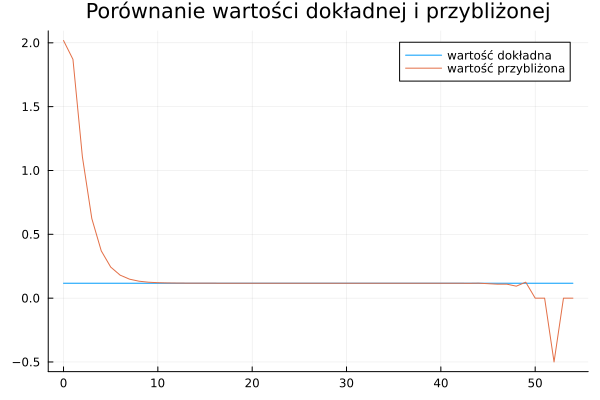
\includegraphics[scale=0.35]{plots/zad7-plot1.png}
    \caption{Obliczone wartości dokładne i przybliżone}
\end{figure}

\begin{figure}[h!]
    \centering
    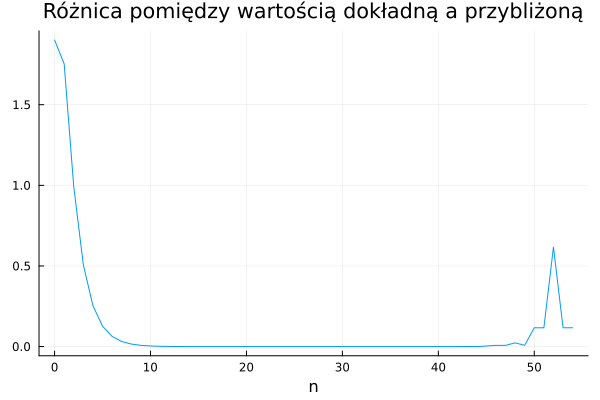
\includegraphics[scale=0.35]{plots/zad7-plot2.png}
    \caption{Błąd pomiędzy wartością dokładną a obliczoną}
\end{figure}

\newpage

\begin{figure}[h!]
    \centering
    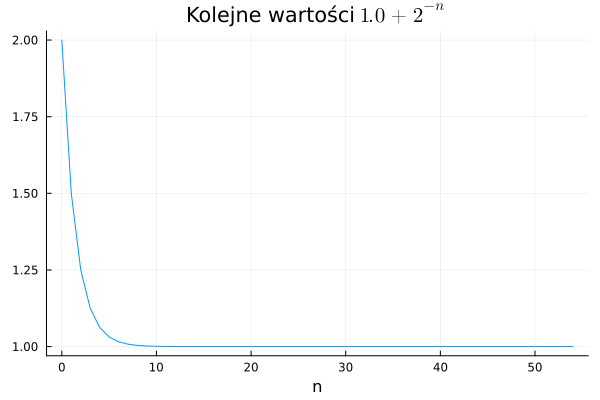
\includegraphics[scale=0.35]{plots/zad7-plot0.png}
    \caption{Badanie wartości $1.0 + h$}
\end{figure}

Początkowe zmiejszanie wartości $h$ poprawia jakość przybliżenia. Jednak gdy $n$ jest przewyższa $40$ błąd rośnie. Powodem takiego zachowania może być fakt, że dodawanie małej wartości do $1.0$ nie zwiększa znacząco jej wartości przez co odejmowane są liczby bliskie siebie c generuje duży błąd.
Dodatkowo dzielenie przez bardzo małe wartości powiększa błąd.

\end{document}
